\documentclass[10pt]{article}
\usepackage[margin=0.8in]{geometry}
\usepackage[T1]{fontenc}
\usepackage{amsmath,amssymb,booktabs,longtable,hyperref,tikz}
\usetikzlibrary{arrows.meta,positioning}
\hypersetup{colorlinks=true,urlcolor=blue}
\title{The Forty W33 Optical Buses:\\
A Restricted Four-MZI XOR Compiler and Coherent Phase-Frame Blueprint}
\author{W33-Theory engineering research}
\date{23 October 2026; mathematical and software evidence}
\begin{document}\maketitle
\begin{abstract}
The previous 40-child fractal Holonet compiler provides forty 4-port line
buses, three XOR-switching states, and a verified three-slot schedule.
We lower each bus to two layers of two ideal Mach--Zehnder (MZI) switching
cells, producing exactly the required 4x4 port permutations up to a
known common optical phase. That yields 160 abstract MZI cells for all
40 buses versus 240 two-mode units in a generic 4x4 unitary-mesh
baseline. We additionally enumerate all W33 pairs of alternative
two-hop routes and expose coherent relative phase mismatches.
This is not a fabricated device, quantum processor, or foundry DRC result.
\end{abstract}
\tableofcontents

\section{Prior art and the limited new contribution}
The W33 graph has 40 vertices, 240 undirected edges, and forty
four-point isotropic lines. Earlier repository work in
\texttt{analysis/w33\_scheduler\_os.py} already exhibited the
forty line buses and a 12-perfect-matching link schedule.
The prior \texttt{analysis/w33\_fractal\_linebus\_switch\_matrix\_20261023.py}
identified the three nonidentity XOR permutations of each four-port bus.
The new work is the executable four-MZI \emph{restricted} circuit
lowering, complete stage/port/virtual-driver manifest, and modulo-four
coherent path phase witness. Four-MZI 4x4 optical switches already
exist in published work; see Sun et al. (2019),
\url{https://www.sciencedirect.com/science/article/abs/pii/S0030399219300702}.
Song et al. (OFC 2021),
\url{https://opg.optica.org/abstract.cfm?URI=OFC-2021-Tu5B.3},
demonstrate why physical phase error and crosstalk still matter.

\section{Exact restricted two-stage transfer}
Let the ideal balanced MZI have
\[
M(\theta)=
\begin{pmatrix}
\cos(\theta/2)&i\sin(\theta/2)\\
i\sin(\theta/2)&\cos(\theta/2)
\end{pmatrix},\qquad
M(0)=I_2,\quad M(\pi)=iX.
\]
The first optical stage comprises switches acting in parallel on
mode pairs $(0,1)$ and $(2,3)$. The second stage comprises
switches acting in parallel on pairs $(0,2)$ and $(1,3)$.
The low mask bit $a\in\{0,1\}$ drives stage one;
the high bit $b\in\{0,1\}$ drives stage two.
For mask $m=a+2b$, the transfer is
\[
U_m=
 \left[M_{02}(\pi b)M_{13}(\pi b)\right]
 \left[M_{01}(\pi a)M_{23}(\pi a)\right]
 =i^{a+b}P_m,\qquad
 (P_m)_{kj}=\delta_{k,j\oplus m}.
\]
This is exact for the defined lossless component convention.
The scalar $i^{a+b}$ must be tracked if different buses or paths
interfere coherently. Multiplying by $i^{-(a+b)}$ restores the target
permutation algebraically; whether it can be corrected virtually,
or needs a real optical reference/phase actuator, depends on
the experimental preparation and interference protocol.
\begin{center}
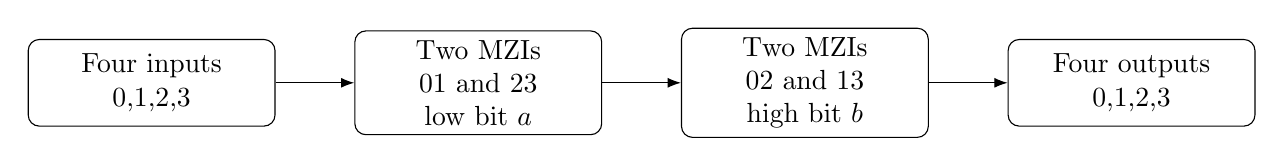
\begin{tikzpicture}[>=Latex,node distance=10mm,
blk/.style={draw,rounded corners,align=center,text width=29mm,minimum height=11mm}]
\node[blk](a){Four inputs\\0,1,2,3};
\node[blk,right=of a](b){Two MZIs\\01 and 23\\low bit $a$};
\node[blk,right=of b](c){Two MZIs\\02 and 13\\high bit $b$};
\node[blk,right=of c](d){Four outputs\\0,1,2,3};
\draw[->](a)--(b);\draw[->](b)--(c);\draw[->](c)--(d);
\end{tikzpicture}
\end{center}
The second-stage nonadjacent mode pairings require actual waveguide
placement and potentially crossings; the diagram is not a photonic
layout. Only four permutations are offered out of $4!=24$:
this is not an unrestricted 4x4 unitary or nonblocking switch.

\section{Device counts and complete machine-readable I/O}
Every four-port line bus has four separately named MZI
devices and two logical stage-control words. In the complete
40-bus parent,
\[
N_{\rm MZI}=40\times4=160,\qquad
N_{\rm logical\ stage\ words}=40\times2=80.
\]
Each stage bit is logically broadcast to both MZIs in its
pair. Individual MZI trim channels and real electrodes might
still be needed for fabrication offsets. The JSON contract names
all four optical ports, every interstage optical net,
160 unassigned electrode IDs, 80 stage words, and all three
slot commands. A general 4x4 unitary mesh has six two-mode
mixers per four-port block, or 240 over 40 blocks. The
restricted topology therefore has one-third fewer \emph{mode
mixer instances}, not necessarily one-third less wafer
area, power, cost or optical loss.

A simplistic loss model assigns $\ell_M$ dB per MZI and
$\ell_X$ dB to the interstage optical crossing/routing
overhead, for equal per-path optical loss
$\ell=2\ell_M+\ell_X$. At the explicitly \emph{hypothetical}
values $\ell_M=0.2$ dB and $\ell_X=0.1$ dB, every ideal
switch path has 0.5 dB modeled loss and roughly
89.1 percent selected power transmission. Distinct random
device errors may break this equality. These numbers are
illustrative; no PIC component data are available.

\section{Why the optical phase frame cannot be ignored}
For ideal mask $m$ define $s(m)=i^{w(m)}$, where $w(m)$
is the two-bit Hamming weight. The physically convenient
MZI gauge yields
\[
s(a)s(b)=(-1)^{w(a\wedge b)}s(a\oplus b).
\]
This scalar defect is a trivializable projective cocycle
of the chosen representation. It does not by itself
represent new topology or quantum-gravitational physics.
For a path with edge masks $m_j$ the optical scalar is
\[
i^e,\qquad e=\left(\sum_jw(m_j)\right)\bmod4.
\]
Crucial: the reciprocal $iX$ amplitude is $i$ in both
forward and reverse directions, so a two-hop round trip
can have phase $-1$. The symmetric edge phase is therefore
not a conventional antisymmetric discrete U(1) gauge connection;
its cycle sums must not be presented as gauge-invariant
Wilson loops.

The exhaustive W33 census has 540 nonadjacent point pairs.
Each has four two-hop routes, giving $540\binom42=3240$
unordered path comparisons. Using the frozen local
line-port ordering, the relative scalar factors are:
\begin{center}
\begin{tabular}{rrr}
\toprule
Exponent difference & Relative factor & Comparisons\\\midrule
0 & $1$ & 1416\\
1 & $i$ & 732\\
2 & $-1$ & 384\\
3 & $-i$ & 708\\\bottomrule
\end{tabular}
\end{center}
For example, routes $0\to4\to7$ and $0\to14\to7$
have scalar phases differing by $i$. All 160 triangles
have zero total scalar exponent in this chosen convention.
These facts are exact results of the finite circuit model,
not an experimental quantum interference measurement and
not invariant under arbitrary physical reference conventions.
A two-arm coherence experiment should test such a difference
with a stable phase reference and calibrated preparation
and measurement errors.

\section{Hardware validation gates}
\begin{longtable}{p{0.30\linewidth}p{0.54\linewidth}}
\toprule
Design boundary & Necessary engineering evidence\\\midrule
Foundry optical network & Actual PDK waveguides, crossings, MZI S-matrices,
layer assignment, DRC and optical connectivity/LVS\\
Electro-optic control & Real electrode maps, bias/phase curves,
individual trimming, drive voltage, bandwidth and cross-talk\\
Coherent-route verification & Measured complex optical transfer,
stable interferometric reference, path-length balancing,
mode dispersion and optical phase noise\\
Quantum characterization & Single-photon source, detector efficiencies,
heralding, interference visibility, calibrated state fidelity\\
Chip packaging & Optical couplers, thermal load, interposer,
electrical pads, drive-channel count and installation constraints\\
\bottomrule
\end{longtable}

\section{Reproducible evidence and software}
The compiler is
\texttt{analysis/w33\_linebus\_xor2\_photonic\_compiler\_20261023.py}
and the path-phase enumerator is
\texttt{analysis/w33\_linebus\_coherent\_path\_phase\_frame\_20261023.py}.
Their outputs are the corresponding \texttt{data/*.json} artifacts.
The two focused \texttt{tests/test\_w33\_linebus*.py} modules
passed 18 tests collectively on 23 October 2026. These
verify exact logical permutations, algebraic scalar
corrections, optical port assignments, an illustrative
loss/error model, and all 3240 alternative-route phase
comparisons. They do not certify fabrication, an optical
test chip, universality or any theory of everything.
\end{document}